\documentclass[twoside]{book}

% Packages required by doxygen
\usepackage{fixltx2e}
\usepackage{calc}
\usepackage{doxygen}
\usepackage[export]{adjustbox} % also loads graphicx
\usepackage{graphicx}
\usepackage[utf8]{inputenc}
\usepackage{makeidx}
\usepackage{multicol}
\usepackage{multirow}
\PassOptionsToPackage{warn}{textcomp}
\usepackage{textcomp}
\usepackage[nointegrals]{wasysym}
\usepackage[table]{xcolor}

% NLS support packages
\usepackage[french]{babel}

% Font selection
\usepackage[T1]{fontenc}
\usepackage[scaled=.90]{helvet}
\usepackage{courier}
\usepackage{amssymb}
\usepackage{sectsty}
\renewcommand{\familydefault}{\sfdefault}
\allsectionsfont{%
  \fontseries{bc}\selectfont%
  \color{darkgray}%
}
\renewcommand{\DoxyLabelFont}{%
  \fontseries{bc}\selectfont%
  \color{darkgray}%
}
\newcommand{\+}{\discretionary{\mbox{\scriptsize$\hookleftarrow$}}{}{}}

% Page & text layout
\usepackage{geometry}
\geometry{%
  a4paper,%
  top=2.5cm,%
  bottom=2.5cm,%
  left=2.5cm,%
  right=2.5cm%
}
\tolerance=750
\hfuzz=15pt
\hbadness=750
\setlength{\emergencystretch}{15pt}
\setlength{\parindent}{0cm}
\setlength{\parskip}{3ex plus 2ex minus 2ex}
\makeatletter
\renewcommand{\paragraph}{%
  \@startsection{paragraph}{4}{0ex}{-1.0ex}{1.0ex}{%
    \normalfont\normalsize\bfseries\SS@parafont%
  }%
}
\renewcommand{\subparagraph}{%
  \@startsection{subparagraph}{5}{0ex}{-1.0ex}{1.0ex}{%
    \normalfont\normalsize\bfseries\SS@subparafont%
  }%
}
\makeatother

% Headers & footers
\usepackage{fancyhdr}
\pagestyle{fancyplain}
\fancyhead[LE]{\fancyplain{}{\bfseries\thepage}}
\fancyhead[CE]{\fancyplain{}{}}
\fancyhead[RE]{\fancyplain{}{\bfseries\leftmark}}
\fancyhead[LO]{\fancyplain{}{\bfseries\rightmark}}
\fancyhead[CO]{\fancyplain{}{}}
\fancyhead[RO]{\fancyplain{}{\bfseries\thepage}}
\fancyfoot[LE]{\fancyplain{}{}}
\fancyfoot[CE]{\fancyplain{}{}}
\fancyfoot[RE]{\fancyplain{}{\bfseries\scriptsize Généré par Doxygen }}
\fancyfoot[LO]{\fancyplain{}{\bfseries\scriptsize Généré par Doxygen }}
\fancyfoot[CO]{\fancyplain{}{}}
\fancyfoot[RO]{\fancyplain{}{}}
\renewcommand{\footrulewidth}{0.4pt}
\renewcommand{\chaptermark}[1]{%
  \markboth{#1}{}%
}
\renewcommand{\sectionmark}[1]{%
  \markright{\thesection\ #1}%
}

% Indices & bibliography
\usepackage{natbib}
\usepackage[titles]{tocloft}
\setcounter{tocdepth}{3}
\setcounter{secnumdepth}{5}
\makeindex

% Hyperlinks (required, but should be loaded last)
\usepackage{ifpdf}
\ifpdf
  \usepackage[pdftex,pagebackref=true]{hyperref}
\else
  \usepackage[ps2pdf,pagebackref=true]{hyperref}
\fi
\hypersetup{%
  colorlinks=true,%
  linkcolor=blue,%
  citecolor=blue,%
  unicode%
}

% Custom commands
\newcommand{\clearemptydoublepage}{%
  \newpage{\pagestyle{empty}\cleardoublepage}%
}

\usepackage{caption}
\captionsetup{labelsep=space,justification=centering,font={bf},singlelinecheck=off,skip=4pt,position=top}

%===== C O N T E N T S =====

\begin{document}

% Titlepage & ToC
\hypersetup{pageanchor=false,
             bookmarksnumbered=true,
             pdfencoding=unicode
            }
\pagenumbering{alph}
\begin{titlepage}
\vspace*{7cm}
\begin{center}%
{\Large Vitesse Acceleration \\[1ex]\large V1.\+0 }\\
\vspace*{1cm}
{\large Généré par Doxygen 1.8.13}\\
\end{center}
\end{titlepage}
\clearemptydoublepage
\pagenumbering{roman}
\tableofcontents
\clearemptydoublepage
\pagenumbering{arabic}
\hypersetup{pageanchor=true}

%--- Begin generated contents ---
\chapter{Index des structures de données}
\section{Structures de données}
Liste des structures de données avec une brève description \+:\begin{DoxyCompactList}
\item\contentsline{section}{\hyperlink{structBackground}{Background} \\*Struct for background }{\pageref{structBackground}}{}
\item\contentsline{section}{\hyperlink{structText}{Text} \\*Struct for \hyperlink{structText}{Text} }{\pageref{structText}}{}
\item\contentsline{section}{\hyperlink{structTime}{Time} \\*Struct for \hyperlink{structTime}{Time} }{\pageref{structTime}}{}
\item\contentsline{section}{\hyperlink{structVoiture}{Voiture} \\*Struct for \hyperlink{structVoiture}{Voiture} }{\pageref{structVoiture}}{}
\end{DoxyCompactList}

\chapter{Index des fichiers}
\input{files}
\chapter{Documentation des structures de données}
\hypertarget{structBackground}{}\section{Référence de la structure Background}
\label{structBackground}\index{Background@{Background}}


struct for background  




{\ttfamily \#include $<$background.\+h$>$}

\subsection*{Champs de données}
\begin{DoxyCompactItemize}
\item 
S\+D\+L\+\_\+\+Surface $\ast$ \hyperlink{structBackground_a13df092f4ec6aebf0364559926479761}{back\+\_\+\+Img}
\item 
S\+D\+L\+\_\+\+Surface $\ast$ \hyperlink{structBackground_a43f21e56f1aa47666ffb4afb34d71cf7}{back\+\_\+\+Img2}
\item 
S\+D\+L\+\_\+\+Rect \hyperlink{structBackground_a4921effe7d9612c8a1870bee947e4441}{back\+\_\+\+Pos}
\end{DoxyCompactItemize}


\subsection{Description détaillée}
struct for background 

\subsection{Documentation des champs}
\mbox{\Hypertarget{structBackground_a13df092f4ec6aebf0364559926479761}\label{structBackground_a13df092f4ec6aebf0364559926479761}} 
\index{Background@{Background}!back\+\_\+\+Img@{back\+\_\+\+Img}}
\index{back\+\_\+\+Img@{back\+\_\+\+Img}!Background@{Background}}
\subsubsection{\texorpdfstring{back\+\_\+\+Img}{back\_Img}}
{\footnotesize\ttfamily S\+D\+L\+\_\+\+Surface$\ast$ Background\+::back\+\_\+\+Img}

Surface. \mbox{\Hypertarget{structBackground_a43f21e56f1aa47666ffb4afb34d71cf7}\label{structBackground_a43f21e56f1aa47666ffb4afb34d71cf7}} 
\index{Background@{Background}!back\+\_\+\+Img2@{back\+\_\+\+Img2}}
\index{back\+\_\+\+Img2@{back\+\_\+\+Img2}!Background@{Background}}
\subsubsection{\texorpdfstring{back\+\_\+\+Img2}{back\_Img2}}
{\footnotesize\ttfamily S\+D\+L\+\_\+\+Surface$\ast$ Background\+::back\+\_\+\+Img2}

Surface. \mbox{\Hypertarget{structBackground_a4921effe7d9612c8a1870bee947e4441}\label{structBackground_a4921effe7d9612c8a1870bee947e4441}} 
\index{Background@{Background}!back\+\_\+\+Pos@{back\+\_\+\+Pos}}
\index{back\+\_\+\+Pos@{back\+\_\+\+Pos}!Background@{Background}}
\subsubsection{\texorpdfstring{back\+\_\+\+Pos}{back\_Pos}}
{\footnotesize\ttfamily S\+D\+L\+\_\+\+Rect Background\+::back\+\_\+\+Pos}

Rectangle 

La documentation de cette structure a été générée à partir du fichier suivant \+:\begin{DoxyCompactItemize}
\item 
\hyperlink{background_8h}{background.\+h}\end{DoxyCompactItemize}

\hypertarget{structText}{}\section{Référence de la structure Text}
\label{structText}\index{Text@{Text}}


struct for \hyperlink{structText}{Text}  




{\ttfamily \#include $<$text.\+h$>$}

\subsection*{Champs de données}
\begin{DoxyCompactItemize}
\item 
S\+D\+L\+\_\+\+Surface $\ast$ \hyperlink{structText_aa9f1ddd6c46522be1712d469256e81ea}{text\+Dt}
\item 
S\+D\+L\+\_\+\+Surface $\ast$ \hyperlink{structText_aaaecac8acfd75d3d856eadb3f887beb7}{text\+\_\+\+Position}
\item 
S\+D\+L\+\_\+\+Surface $\ast$ \hyperlink{structText_ad63fdcfb9a101546a60594eed8cac3e1}{text\+\_\+\+Vitesse}
\item 
S\+D\+L\+\_\+\+Surface $\ast$ \hyperlink{structText_a9c3acebc81d4aa6cbed1a3f75e0c8ea3}{text\+\_\+\+Acceleration}
\end{DoxyCompactItemize}


\subsection{Description détaillée}
struct for \hyperlink{structText}{Text} 

\subsection{Documentation des champs}
\mbox{\Hypertarget{structText_a9c3acebc81d4aa6cbed1a3f75e0c8ea3}\label{structText_a9c3acebc81d4aa6cbed1a3f75e0c8ea3}} 
\index{Text@{Text}!text\+\_\+\+Acceleration@{text\+\_\+\+Acceleration}}
\index{text\+\_\+\+Acceleration@{text\+\_\+\+Acceleration}!Text@{Text}}
\subsubsection{\texorpdfstring{text\+\_\+\+Acceleration}{text\_Acceleration}}
{\footnotesize\ttfamily S\+D\+L\+\_\+\+Surface$\ast$ Text\+::text\+\_\+\+Acceleration}

Surface. \mbox{\Hypertarget{structText_aaaecac8acfd75d3d856eadb3f887beb7}\label{structText_aaaecac8acfd75d3d856eadb3f887beb7}} 
\index{Text@{Text}!text\+\_\+\+Position@{text\+\_\+\+Position}}
\index{text\+\_\+\+Position@{text\+\_\+\+Position}!Text@{Text}}
\subsubsection{\texorpdfstring{text\+\_\+\+Position}{text\_Position}}
{\footnotesize\ttfamily S\+D\+L\+\_\+\+Surface$\ast$ Text\+::text\+\_\+\+Position}

Surface. \mbox{\Hypertarget{structText_ad63fdcfb9a101546a60594eed8cac3e1}\label{structText_ad63fdcfb9a101546a60594eed8cac3e1}} 
\index{Text@{Text}!text\+\_\+\+Vitesse@{text\+\_\+\+Vitesse}}
\index{text\+\_\+\+Vitesse@{text\+\_\+\+Vitesse}!Text@{Text}}
\subsubsection{\texorpdfstring{text\+\_\+\+Vitesse}{text\_Vitesse}}
{\footnotesize\ttfamily S\+D\+L\+\_\+\+Surface$\ast$ Text\+::text\+\_\+\+Vitesse}

Surface. \mbox{\Hypertarget{structText_aa9f1ddd6c46522be1712d469256e81ea}\label{structText_aa9f1ddd6c46522be1712d469256e81ea}} 
\index{Text@{Text}!text\+Dt@{text\+Dt}}
\index{text\+Dt@{text\+Dt}!Text@{Text}}
\subsubsection{\texorpdfstring{text\+Dt}{textDt}}
{\footnotesize\ttfamily S\+D\+L\+\_\+\+Surface$\ast$ Text\+::text\+Dt}

Surface. 

La documentation de cette structure a été générée à partir du fichier suivant \+:\begin{DoxyCompactItemize}
\item 
\hyperlink{text_8h}{text.\+h}\end{DoxyCompactItemize}

\hypertarget{structTime}{}\section{Référence de la structure Time}
\label{structTime}\index{Time@{Time}}


struct for \hyperlink{structTime}{Time}  




{\ttfamily \#include $<$text.\+h$>$}

\subsection*{Champs de données}
\begin{DoxyCompactItemize}
\item 
S\+D\+L\+\_\+\+Surface $\ast$ \hyperlink{structTime_a75df5e60edca4a4555029589f430f72e}{msg}
\item 
T\+T\+F\+\_\+\+Font $\ast$ \hyperlink{structTime_a870d34231ad11f87e284a0fd74b22f33}{font}
\item 
int \hyperlink{structTime_a11f3327ad1d256262bfa22b7e0553b60}{temps}
\item 
char \hyperlink{structTime_a6d30063c4d2f746ce34949138a2be479}{time\+String} \mbox{[}10\mbox{]}
\end{DoxyCompactItemize}


\subsection{Description détaillée}
struct for \hyperlink{structTime}{Time} 

\subsection{Documentation des champs}
\mbox{\Hypertarget{structTime_a870d34231ad11f87e284a0fd74b22f33}\label{structTime_a870d34231ad11f87e284a0fd74b22f33}} 
\index{Time@{Time}!font@{font}}
\index{font@{font}!Time@{Time}}
\subsubsection{\texorpdfstring{font}{font}}
{\footnotesize\ttfamily T\+T\+F\+\_\+\+Font$\ast$ Time\+::font}

Police. \mbox{\Hypertarget{structTime_a75df5e60edca4a4555029589f430f72e}\label{structTime_a75df5e60edca4a4555029589f430f72e}} 
\index{Time@{Time}!msg@{msg}}
\index{msg@{msg}!Time@{Time}}
\subsubsection{\texorpdfstring{msg}{msg}}
{\footnotesize\ttfamily S\+D\+L\+\_\+\+Surface$\ast$ Time\+::msg}

Surface. \mbox{\Hypertarget{structTime_a11f3327ad1d256262bfa22b7e0553b60}\label{structTime_a11f3327ad1d256262bfa22b7e0553b60}} 
\index{Time@{Time}!temps@{temps}}
\index{temps@{temps}!Time@{Time}}
\subsubsection{\texorpdfstring{temps}{temps}}
{\footnotesize\ttfamily int Time\+::temps}

\mbox{\Hypertarget{structTime_a6d30063c4d2f746ce34949138a2be479}\label{structTime_a6d30063c4d2f746ce34949138a2be479}} 
\index{Time@{Time}!time\+String@{time\+String}}
\index{time\+String@{time\+String}!Time@{Time}}
\subsubsection{\texorpdfstring{time\+String}{timeString}}
{\footnotesize\ttfamily char Time\+::time\+String\mbox{[}10\mbox{]}}



La documentation de cette structure a été générée à partir du fichier suivant \+:\begin{DoxyCompactItemize}
\item 
\hyperlink{text_8h}{text.\+h}\end{DoxyCompactItemize}

\hypertarget{structVoiture}{}\section{Référence de la structure Voiture}
\label{structVoiture}\index{Voiture@{Voiture}}


struct for \hyperlink{structVoiture}{Voiture}  




{\ttfamily \#include $<$voiture.\+h$>$}

\subsection*{Champs de données}
\begin{DoxyCompactItemize}
\item 
S\+D\+L\+\_\+\+Rect \hyperlink{structVoiture_a68748b5ea1dfc3d0d2797f675e03f139}{position}
\item 
S\+D\+L\+\_\+\+Surface $\ast$ \hyperlink{structVoiture_aeeb926bfdf6133f6c0e4e7c6c1a09394}{image} \mbox{[}5\mbox{]}
\item 
int \hyperlink{structVoiture_a9bb35d6796c9a008309a574e14984227}{direction}
\item 
int \hyperlink{structVoiture_a71f00083102cac3802ca4fc5686c9b28}{move}
\item 
float \hyperlink{structVoiture_a017e4fa03a51b03bbf72232bf33fa2f7}{Mass}
\item 
double \hyperlink{structVoiture_ad4b4d14b11ebddd488eda893e3438bb3}{vitesse}
\item 
double \hyperlink{structVoiture_a9774aa8f724f65d16b7d0104e1ed8ecd}{acceleration}
\end{DoxyCompactItemize}


\subsection{Description détaillée}
struct for \hyperlink{structVoiture}{Voiture} 

\subsection{Documentation des champs}
\mbox{\Hypertarget{structVoiture_a9774aa8f724f65d16b7d0104e1ed8ecd}\label{structVoiture_a9774aa8f724f65d16b7d0104e1ed8ecd}} 
\index{Voiture@{Voiture}!acceleration@{acceleration}}
\index{acceleration@{acceleration}!Voiture@{Voiture}}
\subsubsection{\texorpdfstring{acceleration}{acceleration}}
{\footnotesize\ttfamily double Voiture\+::acceleration}

\mbox{\Hypertarget{structVoiture_a9bb35d6796c9a008309a574e14984227}\label{structVoiture_a9bb35d6796c9a008309a574e14984227}} 
\index{Voiture@{Voiture}!direction@{direction}}
\index{direction@{direction}!Voiture@{Voiture}}
\subsubsection{\texorpdfstring{direction}{direction}}
{\footnotesize\ttfamily int Voiture\+::direction}

\mbox{\Hypertarget{structVoiture_aeeb926bfdf6133f6c0e4e7c6c1a09394}\label{structVoiture_aeeb926bfdf6133f6c0e4e7c6c1a09394}} 
\index{Voiture@{Voiture}!image@{image}}
\index{image@{image}!Voiture@{Voiture}}
\subsubsection{\texorpdfstring{image}{image}}
{\footnotesize\ttfamily S\+D\+L\+\_\+\+Surface$\ast$ Voiture\+::image\mbox{[}5\mbox{]}}

Surface. \mbox{\Hypertarget{structVoiture_a017e4fa03a51b03bbf72232bf33fa2f7}\label{structVoiture_a017e4fa03a51b03bbf72232bf33fa2f7}} 
\index{Voiture@{Voiture}!Mass@{Mass}}
\index{Mass@{Mass}!Voiture@{Voiture}}
\subsubsection{\texorpdfstring{Mass}{Mass}}
{\footnotesize\ttfamily float Voiture\+::\+Mass}

\mbox{\Hypertarget{structVoiture_a71f00083102cac3802ca4fc5686c9b28}\label{structVoiture_a71f00083102cac3802ca4fc5686c9b28}} 
\index{Voiture@{Voiture}!move@{move}}
\index{move@{move}!Voiture@{Voiture}}
\subsubsection{\texorpdfstring{move}{move}}
{\footnotesize\ttfamily int Voiture\+::move}

\mbox{\Hypertarget{structVoiture_a68748b5ea1dfc3d0d2797f675e03f139}\label{structVoiture_a68748b5ea1dfc3d0d2797f675e03f139}} 
\index{Voiture@{Voiture}!position@{position}}
\index{position@{position}!Voiture@{Voiture}}
\subsubsection{\texorpdfstring{position}{position}}
{\footnotesize\ttfamily S\+D\+L\+\_\+\+Rect Voiture\+::position}

Rectangle \mbox{\Hypertarget{structVoiture_ad4b4d14b11ebddd488eda893e3438bb3}\label{structVoiture_ad4b4d14b11ebddd488eda893e3438bb3}} 
\index{Voiture@{Voiture}!vitesse@{vitesse}}
\index{vitesse@{vitesse}!Voiture@{Voiture}}
\subsubsection{\texorpdfstring{vitesse}{vitesse}}
{\footnotesize\ttfamily double Voiture\+::vitesse}



La documentation de cette structure a été générée à partir du fichier suivant \+:\begin{DoxyCompactItemize}
\item 
\hyperlink{voiture_8h}{voiture.\+h}\end{DoxyCompactItemize}

\chapter{Documentation des fichiers}
\hypertarget{background_8c}{}\section{Référence du fichier background.\+c}
\label{background_8c}\index{background.\+c@{background.\+c}}
{\ttfamily \#include \char`\"{}background.\+h\char`\"{}}\newline
{\ttfamily \#include \char`\"{}text.\+h\char`\"{}}\newline
Graphe des dépendances par inclusion de background.\+c\+:
\nopagebreak
\begin{figure}[H]
\begin{center}
\leavevmode
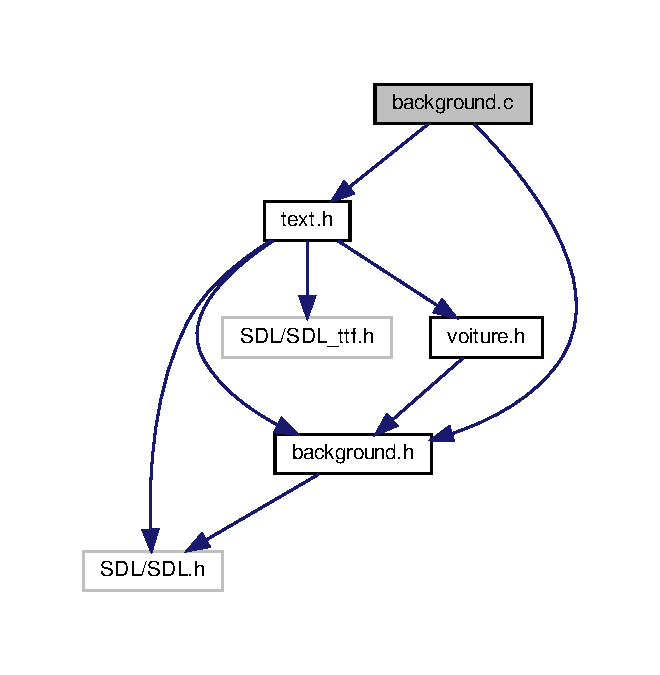
\includegraphics[width=317pt]{background_8c__incl}
\end{center}
\end{figure}
\subsection*{Fonctions}
\begin{DoxyCompactItemize}
\item 
void \hyperlink{background_8c_a7690baf8498d427ca7dbb6ff0f06b142}{load\+Background} (\hyperlink{structBackground}{Background} $\ast$Back)
\begin{DoxyCompactList}\small\item\em Load \hyperlink{structBackground}{Background} Back. \end{DoxyCompactList}\item 
void \hyperlink{background_8c_a80c8e2751f2e1049fe1c033f2a971fe0}{init\+Background} (\hyperlink{structBackground}{Background} $\ast$Back)
\begin{DoxyCompactList}\small\item\em initialiser \hyperlink{structBackground}{Background} Back. \end{DoxyCompactList}\item 
void \hyperlink{background_8c_acd20976661c4bf621c809bf465f59f68}{blit\+Background} (\hyperlink{structBackground}{Background} $\ast$Back, S\+D\+L\+\_\+\+Surface $\ast$screen)
\begin{DoxyCompactList}\small\item\em Afficher le background back . \end{DoxyCompactList}\item 
void \hyperlink{background_8c_a04645de4c3c73cae976c1ceb1fe06548}{free\+Background} (\hyperlink{structBackground}{Background} $\ast$Back)
\begin{DoxyCompactList}\small\item\em Liberer la surface. \end{DoxyCompactList}\end{DoxyCompactItemize}


\subsection{Documentation des fonctions}
\mbox{\Hypertarget{background_8c_acd20976661c4bf621c809bf465f59f68}\label{background_8c_acd20976661c4bf621c809bf465f59f68}} 
\index{background.\+c@{background.\+c}!blit\+Background@{blit\+Background}}
\index{blit\+Background@{blit\+Background}!background.\+c@{background.\+c}}
\subsubsection{\texorpdfstring{blit\+Background()}{blitBackground()}}
{\footnotesize\ttfamily void blit\+Background (\begin{DoxyParamCaption}\item[{\hyperlink{structBackground}{Background} $\ast$}]{Back,  }\item[{S\+D\+L\+\_\+\+Surface $\ast$}]{screen }\end{DoxyParamCaption})}



Afficher le background back . 


\begin{DoxyParams}{Paramètres}
{\em scren} & the screen \\
\hline
{\em back} & the background \\
\hline
\end{DoxyParams}
\begin{DoxyReturn}{Renvoie}
rien 
\end{DoxyReturn}
Voici le graphe des appelants de cette fonction \+:
\nopagebreak
\begin{figure}[H]
\begin{center}
\leavevmode
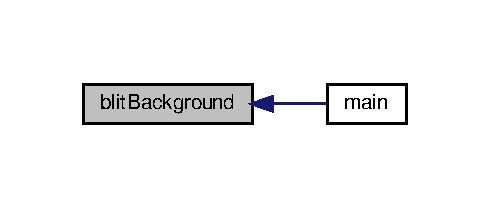
\includegraphics[width=235pt]{background_8c_acd20976661c4bf621c809bf465f59f68_icgraph}
\end{center}
\end{figure}
\mbox{\Hypertarget{background_8c_a04645de4c3c73cae976c1ceb1fe06548}\label{background_8c_a04645de4c3c73cae976c1ceb1fe06548}} 
\index{background.\+c@{background.\+c}!free\+Background@{free\+Background}}
\index{free\+Background@{free\+Background}!background.\+c@{background.\+c}}
\subsubsection{\texorpdfstring{free\+Background()}{freeBackground()}}
{\footnotesize\ttfamily void free\+Background (\begin{DoxyParamCaption}\item[{\hyperlink{structBackground}{Background} $\ast$}]{Back }\end{DoxyParamCaption})}



Liberer la surface. 


\begin{DoxyParams}{Paramètres}
{\em back} & the background \\
\hline
\end{DoxyParams}
\begin{DoxyReturn}{Renvoie}
rien 
\end{DoxyReturn}
Voici le graphe des appelants de cette fonction \+:
\nopagebreak
\begin{figure}[H]
\begin{center}
\leavevmode
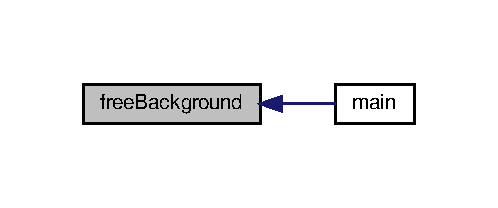
\includegraphics[width=239pt]{background_8c_a04645de4c3c73cae976c1ceb1fe06548_icgraph}
\end{center}
\end{figure}
\mbox{\Hypertarget{background_8c_a80c8e2751f2e1049fe1c033f2a971fe0}\label{background_8c_a80c8e2751f2e1049fe1c033f2a971fe0}} 
\index{background.\+c@{background.\+c}!init\+Background@{init\+Background}}
\index{init\+Background@{init\+Background}!background.\+c@{background.\+c}}
\subsubsection{\texorpdfstring{init\+Background()}{initBackground()}}
{\footnotesize\ttfamily void init\+Background (\begin{DoxyParamCaption}\item[{\hyperlink{structBackground}{Background} $\ast$}]{Back }\end{DoxyParamCaption})}



initialiser \hyperlink{structBackground}{Background} Back. 


\begin{DoxyParams}{Paramètres}
{\em back} & le background \\
\hline
\end{DoxyParams}
\begin{DoxyReturn}{Renvoie}
Rien 
\end{DoxyReturn}
Voici le graphe des appelants de cette fonction \+:
\nopagebreak
\begin{figure}[H]
\begin{center}
\leavevmode
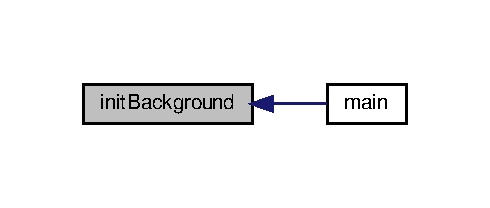
\includegraphics[width=235pt]{background_8c_a80c8e2751f2e1049fe1c033f2a971fe0_icgraph}
\end{center}
\end{figure}
\mbox{\Hypertarget{background_8c_a7690baf8498d427ca7dbb6ff0f06b142}\label{background_8c_a7690baf8498d427ca7dbb6ff0f06b142}} 
\index{background.\+c@{background.\+c}!load\+Background@{load\+Background}}
\index{load\+Background@{load\+Background}!background.\+c@{background.\+c}}
\subsubsection{\texorpdfstring{load\+Background()}{loadBackground()}}
{\footnotesize\ttfamily void load\+Background (\begin{DoxyParamCaption}\item[{\hyperlink{structBackground}{Background} $\ast$}]{Back }\end{DoxyParamCaption})}



Load \hyperlink{structBackground}{Background} Back. 


\begin{DoxyParams}{Paramètres}
{\em back} & le background \\
\hline
\end{DoxyParams}
\begin{DoxyReturn}{Renvoie}
Rien 
\end{DoxyReturn}
Voici le graphe des appelants de cette fonction \+:
\nopagebreak
\begin{figure}[H]
\begin{center}
\leavevmode
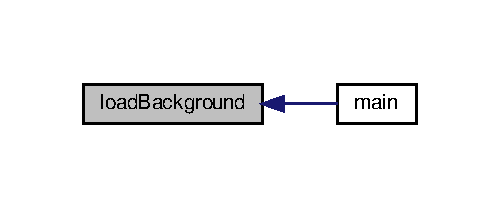
\includegraphics[width=240pt]{background_8c_a7690baf8498d427ca7dbb6ff0f06b142_icgraph}
\end{center}
\end{figure}

\input{background_8h}
\hypertarget{main_8c}{}\section{Référence du fichier main.\+c}
\label{main_8c}\index{main.\+c@{main.\+c}}


Tester programme.  


{\ttfamily \#include $<$stdio.\+h$>$}\newline
{\ttfamily \#include $<$stdlib.\+h$>$}\newline
{\ttfamily \#include $<$S\+D\+L/\+S\+D\+L.\+h$>$}\newline
{\ttfamily \#include \char`\"{}S\+D\+L/\+S\+D\+L\+\_\+image.\+h\char`\"{}}\newline
{\ttfamily \#include $<$S\+D\+L/\+S\+D\+L\+\_\+mixer.\+h$>$}\newline
{\ttfamily \#include \char`\"{}background.\+h\char`\"{}}\newline
{\ttfamily \#include \char`\"{}voiture.\+h\char`\"{}}\newline
{\ttfamily \#include \char`\"{}text.\+h\char`\"{}}\newline
Graphe des dépendances par inclusion de main.\+c\+:
\nopagebreak
\begin{figure}[H]
\begin{center}
\leavevmode
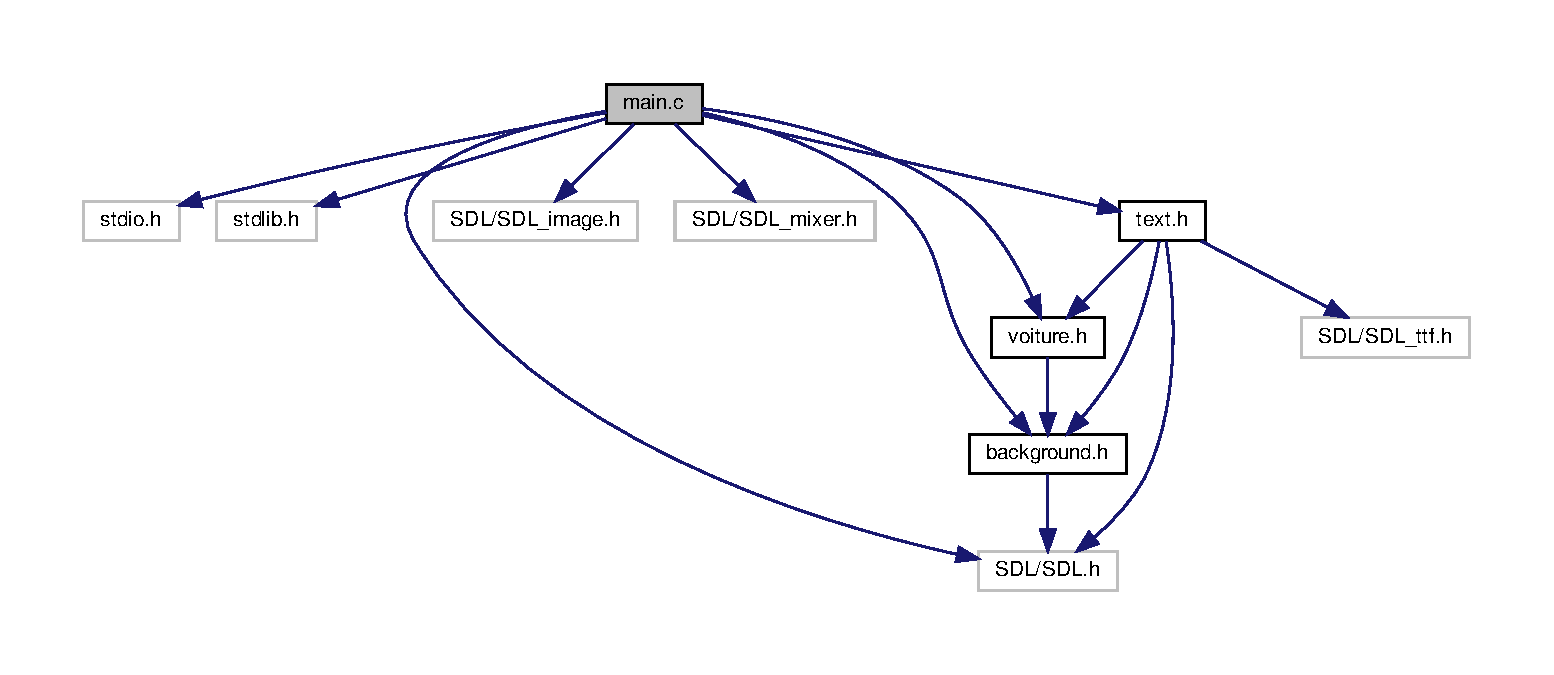
\includegraphics[width=350pt]{main_8c__incl}
\end{center}
\end{figure}
\subsection*{Fonctions}
\begin{DoxyCompactItemize}
\item 
int \hyperlink{main_8c_a840291bc02cba5474a4cb46a9b9566fe}{main} (void)
\end{DoxyCompactItemize}


\subsection{Description détaillée}
Tester programme. 

\begin{DoxyAuthor}{Auteur}
Bechir Mennai 
\end{DoxyAuthor}
\begin{DoxyVersion}{Version}
1.\+0 
\end{DoxyVersion}
\begin{DoxyDate}{Date}
Juin 01, 2020
\end{DoxyDate}
Tester programme pour Vitesse Acceleration 

\subsection{Documentation des fonctions}
\mbox{\Hypertarget{main_8c_a840291bc02cba5474a4cb46a9b9566fe}\label{main_8c_a840291bc02cba5474a4cb46a9b9566fe}} 
\index{main.\+c@{main.\+c}!main@{main}}
\index{main@{main}!main.\+c@{main.\+c}}
\subsubsection{\texorpdfstring{main()}{main()}}
{\footnotesize\ttfamily int main (\begin{DoxyParamCaption}\item[{void}]{ }\end{DoxyParamCaption})}

Voici le graphe d\textquotesingle{}appel pour cette fonction \+:
\nopagebreak
\begin{figure}[H]
\begin{center}
\leavevmode
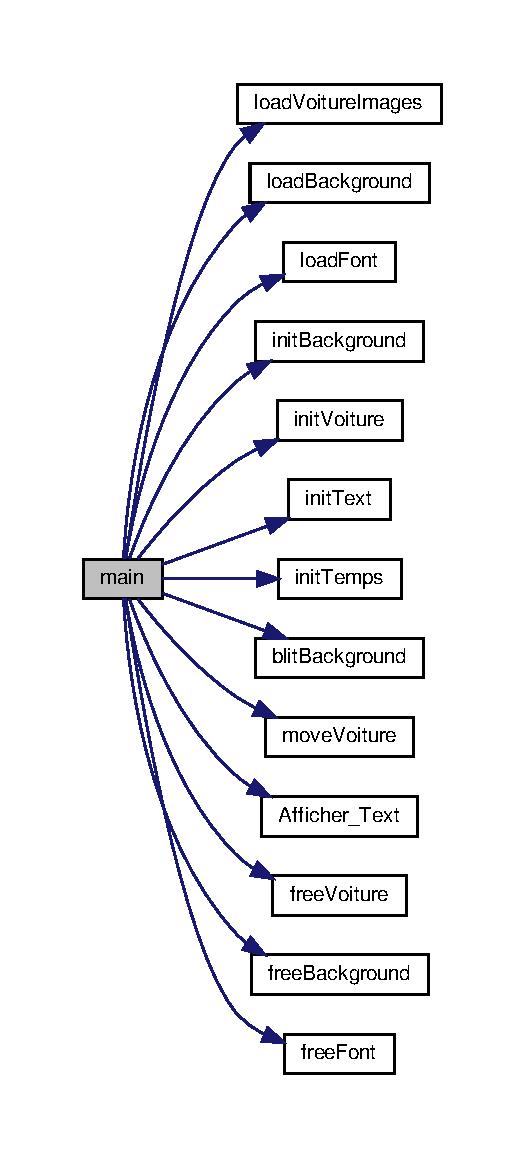
\includegraphics[height=550pt]{main_8c_a840291bc02cba5474a4cb46a9b9566fe_cgraph}
\end{center}
\end{figure}

\hypertarget{text_8c}{}\section{Référence du fichier text.\+c}
\label{text_8c}\index{text.\+c@{text.\+c}}
{\ttfamily \#include \char`\"{}text.\+h\char`\"{}}\newline
Graphe des dépendances par inclusion de text.\+c\+:
\nopagebreak
\begin{figure}[H]
\begin{center}
\leavevmode
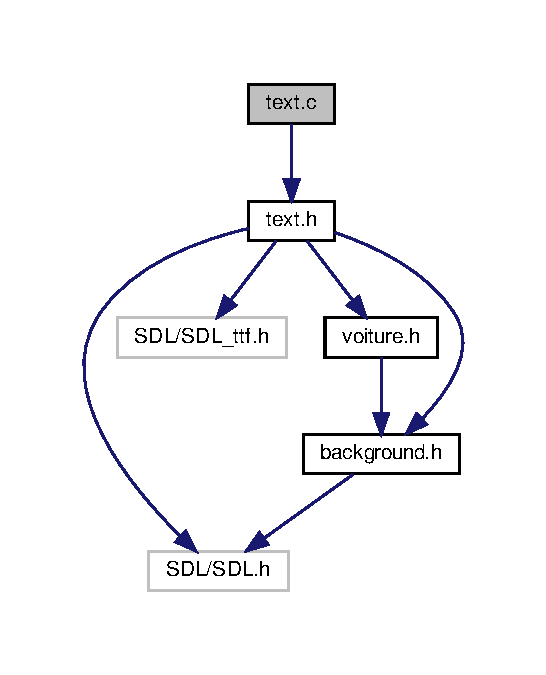
\includegraphics[width=262pt]{text_8c__incl}
\end{center}
\end{figure}
\subsection*{Fonctions}
\begin{DoxyCompactItemize}
\item 
void \hyperlink{text_8c_ab262a155d2f6fdeefc6ad6d63da93c82}{init\+Text} (\hyperlink{structText}{Text} $\ast$T)
\begin{DoxyCompactList}\small\item\em initialiser \hyperlink{structText}{Text} T. \end{DoxyCompactList}\item 
void \hyperlink{text_8c_a2dc500fe2665ba740d37f08e490c2a6a}{init\+Temps} (\hyperlink{structTime}{Time} $\ast$time)
\begin{DoxyCompactList}\small\item\em initialiser \hyperlink{structTime}{Time} time. \end{DoxyCompactList}\item 
void \hyperlink{text_8c_a6f50df17af941d4d1aff8d62c336edca}{load\+Font} (T\+T\+F\+\_\+\+Font $\ast$$\ast$police)
\begin{DoxyCompactList}\small\item\em Load Font. \end{DoxyCompactList}\item 
void \hyperlink{text_8c_a307b7655043a42402d751a3da90ff1d0}{Afficher\+\_\+\+Text} (T\+T\+F\+\_\+\+Font $\ast$police, \hyperlink{structText}{Text} $\ast$T, S\+D\+L\+\_\+\+Surface $\ast$screen, \hyperlink{structVoiture}{Voiture} V, \hyperlink{structBackground}{Background} Back, \hyperlink{structTime}{Time} $\ast$time, Uint32 dt)
\begin{DoxyCompactList}\small\item\em Afficher tout les text . \end{DoxyCompactList}\item 
void \hyperlink{text_8c_aed94d72c6d43ac78f60f25e0d622d3bd}{free\+Font} (T\+T\+F\+\_\+\+Font $\ast$$\ast$police)
\begin{DoxyCompactList}\small\item\em Liberer la surface. \end{DoxyCompactList}\end{DoxyCompactItemize}


\subsection{Documentation des fonctions}
\mbox{\Hypertarget{text_8c_a307b7655043a42402d751a3da90ff1d0}\label{text_8c_a307b7655043a42402d751a3da90ff1d0}} 
\index{text.\+c@{text.\+c}!Afficher\+\_\+\+Text@{Afficher\+\_\+\+Text}}
\index{Afficher\+\_\+\+Text@{Afficher\+\_\+\+Text}!text.\+c@{text.\+c}}
\subsubsection{\texorpdfstring{Afficher\+\_\+\+Text()}{Afficher\_Text()}}
{\footnotesize\ttfamily void Afficher\+\_\+\+Text (\begin{DoxyParamCaption}\item[{T\+T\+F\+\_\+\+Font $\ast$}]{police,  }\item[{\hyperlink{structText}{Text} $\ast$}]{T,  }\item[{S\+D\+L\+\_\+\+Surface $\ast$}]{screen,  }\item[{\hyperlink{structVoiture}{Voiture}}]{V,  }\item[{\hyperlink{structBackground}{Background}}]{Back,  }\item[{\hyperlink{structTime}{Time} $\ast$}]{time,  }\item[{Uint32}]{dt }\end{DoxyParamCaption})}



Afficher tout les text . 


\begin{DoxyParams}{Paramètres}
{\em scren} & the screen \\
\hline
{\em back} & the background \\
\hline
{\em time} & le \hyperlink{structTime}{Time} \\
\hline
{\em police} & le font \\
\hline
{\em T} & le \hyperlink{structText}{Text} \\
\hline
{\em dt} & variation dt \\
\hline
\end{DoxyParams}
\begin{DoxyReturn}{Renvoie}
rien 
\end{DoxyReturn}
Voici le graphe des appelants de cette fonction \+:
\nopagebreak
\begin{figure}[H]
\begin{center}
\leavevmode
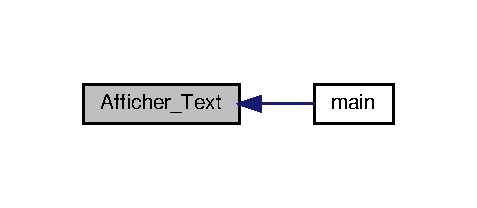
\includegraphics[width=229pt]{text_8c_a307b7655043a42402d751a3da90ff1d0_icgraph}
\end{center}
\end{figure}
\mbox{\Hypertarget{text_8c_aed94d72c6d43ac78f60f25e0d622d3bd}\label{text_8c_aed94d72c6d43ac78f60f25e0d622d3bd}} 
\index{text.\+c@{text.\+c}!free\+Font@{free\+Font}}
\index{free\+Font@{free\+Font}!text.\+c@{text.\+c}}
\subsubsection{\texorpdfstring{free\+Font()}{freeFont()}}
{\footnotesize\ttfamily void free\+Font (\begin{DoxyParamCaption}\item[{T\+T\+F\+\_\+\+Font $\ast$$\ast$}]{police }\end{DoxyParamCaption})}



Liberer la surface. 


\begin{DoxyParams}{Paramètres}
{\em police} & le font \\
\hline
\end{DoxyParams}
\begin{DoxyReturn}{Renvoie}
rien 
\end{DoxyReturn}
Voici le graphe des appelants de cette fonction \+:
\nopagebreak
\begin{figure}[H]
\begin{center}
\leavevmode
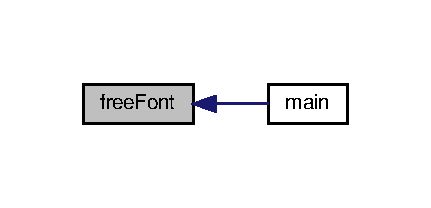
\includegraphics[width=207pt]{text_8c_aed94d72c6d43ac78f60f25e0d622d3bd_icgraph}
\end{center}
\end{figure}
\mbox{\Hypertarget{text_8c_a2dc500fe2665ba740d37f08e490c2a6a}\label{text_8c_a2dc500fe2665ba740d37f08e490c2a6a}} 
\index{text.\+c@{text.\+c}!init\+Temps@{init\+Temps}}
\index{init\+Temps@{init\+Temps}!text.\+c@{text.\+c}}
\subsubsection{\texorpdfstring{init\+Temps()}{initTemps()}}
{\footnotesize\ttfamily void init\+Temps (\begin{DoxyParamCaption}\item[{\hyperlink{structTime}{Time} $\ast$}]{time }\end{DoxyParamCaption})}



initialiser \hyperlink{structTime}{Time} time. 


\begin{DoxyParams}{Paramètres}
{\em time} & le \hyperlink{structTime}{Time} \\
\hline
\end{DoxyParams}
\begin{DoxyReturn}{Renvoie}
Rien 
\end{DoxyReturn}
Voici le graphe des appelants de cette fonction \+:
\nopagebreak
\begin{figure}[H]
\begin{center}
\leavevmode
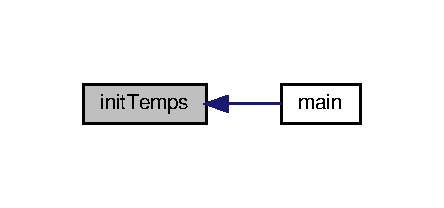
\includegraphics[width=213pt]{text_8c_a2dc500fe2665ba740d37f08e490c2a6a_icgraph}
\end{center}
\end{figure}
\mbox{\Hypertarget{text_8c_ab262a155d2f6fdeefc6ad6d63da93c82}\label{text_8c_ab262a155d2f6fdeefc6ad6d63da93c82}} 
\index{text.\+c@{text.\+c}!init\+Text@{init\+Text}}
\index{init\+Text@{init\+Text}!text.\+c@{text.\+c}}
\subsubsection{\texorpdfstring{init\+Text()}{initText()}}
{\footnotesize\ttfamily void init\+Text (\begin{DoxyParamCaption}\item[{\hyperlink{structText}{Text} $\ast$}]{T }\end{DoxyParamCaption})}



initialiser \hyperlink{structText}{Text} T. 


\begin{DoxyParams}{Paramètres}
{\em T} & le \hyperlink{structText}{Text} \\
\hline
\end{DoxyParams}
\begin{DoxyReturn}{Renvoie}
Rien 
\end{DoxyReturn}
Voici le graphe des appelants de cette fonction \+:
\nopagebreak
\begin{figure}[H]
\begin{center}
\leavevmode
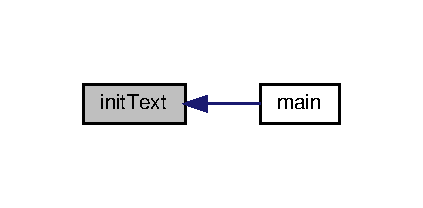
\includegraphics[width=203pt]{text_8c_ab262a155d2f6fdeefc6ad6d63da93c82_icgraph}
\end{center}
\end{figure}
\mbox{\Hypertarget{text_8c_a6f50df17af941d4d1aff8d62c336edca}\label{text_8c_a6f50df17af941d4d1aff8d62c336edca}} 
\index{text.\+c@{text.\+c}!load\+Font@{load\+Font}}
\index{load\+Font@{load\+Font}!text.\+c@{text.\+c}}
\subsubsection{\texorpdfstring{load\+Font()}{loadFont()}}
{\footnotesize\ttfamily void load\+Font (\begin{DoxyParamCaption}\item[{T\+T\+F\+\_\+\+Font $\ast$$\ast$}]{police }\end{DoxyParamCaption})}



Load Font. 


\begin{DoxyParams}{Paramètres}
{\em police} & le font \\
\hline
\end{DoxyParams}
\begin{DoxyReturn}{Renvoie}
Rien 
\end{DoxyReturn}
Voici le graphe des appelants de cette fonction \+:
\nopagebreak
\begin{figure}[H]
\begin{center}
\leavevmode
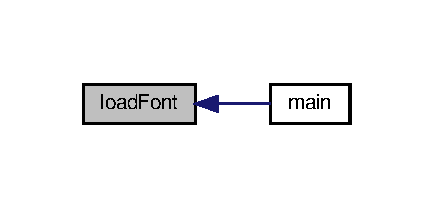
\includegraphics[width=208pt]{text_8c_a6f50df17af941d4d1aff8d62c336edca_icgraph}
\end{center}
\end{figure}

\hypertarget{text_8h}{}\section{Référence du fichier text.\+h}
\label{text_8h}\index{text.\+h@{text.\+h}}
{\ttfamily \#include $<$S\+D\+L/\+S\+D\+L.\+h$>$}\newline
{\ttfamily \#include $<$S\+D\+L/\+S\+D\+L\+\_\+ttf.\+h$>$}\newline
{\ttfamily \#include \char`\"{}voiture.\+h\char`\"{}}\newline
{\ttfamily \#include \char`\"{}background.\+h\char`\"{}}\newline
Graphe des dépendances par inclusion de text.\+h\+:
\nopagebreak
\begin{figure}[H]
\begin{center}
\leavevmode
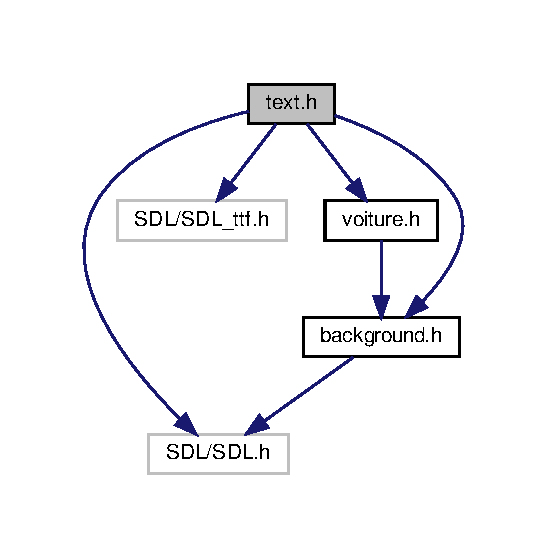
\includegraphics[width=262pt]{text_8h__incl}
\end{center}
\end{figure}
Ce graphe montre quels fichiers incluent directement ou indirectement ce fichier \+:
\nopagebreak
\begin{figure}[H]
\begin{center}
\leavevmode
\includegraphics[width=350pt]{text_8h__dep__incl}
\end{center}
\end{figure}
\subsection*{Structures de données}
\begin{DoxyCompactItemize}
\item 
struct \hyperlink{structText}{Text}
\begin{DoxyCompactList}\small\item\em struct for \hyperlink{structText}{Text} \end{DoxyCompactList}\item 
struct \hyperlink{structTime}{Time}
\begin{DoxyCompactList}\small\item\em struct for \hyperlink{structTime}{Time} \end{DoxyCompactList}\end{DoxyCompactItemize}
\subsection*{Macros}
\begin{DoxyCompactItemize}
\item 
\#define \hyperlink{text_8h_ac92ca5ab87034a348decad7ee8d4bd1b}{F\+PS}~60
\item 
\#define \hyperlink{text_8h_a91023e7c9b297a2cf1ef0728903a4308}{A\+C\+C\+E\+LX}~0
\item 
\#define \hyperlink{text_8h_a7434bdf859f83feeae7473fdf8841c18}{A\+C\+C\+E\+LY}~0
\item 
\#define \hyperlink{text_8h_a9b6bc9242882d1e758e06ed751a2e8ec}{S\+C\+R\+E\+E\+N\+\_\+W}~1000
\item 
\#define \hyperlink{text_8h_a27cddfd509d28b4b2b0b44c093fac090}{S\+C\+R\+E\+E\+N\+\_\+H}~400
\end{DoxyCompactItemize}
\subsection*{Fonctions}
\begin{DoxyCompactItemize}
\item 
void \hyperlink{text_8h_ab262a155d2f6fdeefc6ad6d63da93c82}{init\+Text} (\hyperlink{structText}{Text} $\ast$T)
\begin{DoxyCompactList}\small\item\em initialiser \hyperlink{structText}{Text} T. \end{DoxyCompactList}\item 
void \hyperlink{text_8h_a2dc500fe2665ba740d37f08e490c2a6a}{init\+Temps} (\hyperlink{structTime}{Time} $\ast$time)
\begin{DoxyCompactList}\small\item\em initialiser \hyperlink{structTime}{Time} time. \end{DoxyCompactList}\item 
void \hyperlink{text_8h_a6f50df17af941d4d1aff8d62c336edca}{load\+Font} (T\+T\+F\+\_\+\+Font $\ast$$\ast$police)
\begin{DoxyCompactList}\small\item\em Load Font. \end{DoxyCompactList}\item 
void \hyperlink{text_8h_a307b7655043a42402d751a3da90ff1d0}{Afficher\+\_\+\+Text} (T\+T\+F\+\_\+\+Font $\ast$police, \hyperlink{structText}{Text} $\ast$T, S\+D\+L\+\_\+\+Surface $\ast$screen, \hyperlink{structVoiture}{Voiture} V, \hyperlink{structBackground}{Background} Back, \hyperlink{structTime}{Time} $\ast$time, Uint32 dt)
\begin{DoxyCompactList}\small\item\em Afficher tout les text . \end{DoxyCompactList}\item 
void \hyperlink{text_8h_aed94d72c6d43ac78f60f25e0d622d3bd}{free\+Font} (T\+T\+F\+\_\+\+Font $\ast$$\ast$police)
\begin{DoxyCompactList}\small\item\em Liberer la surface. \end{DoxyCompactList}\end{DoxyCompactItemize}


\subsection{Documentation des macros}
\mbox{\Hypertarget{text_8h_a91023e7c9b297a2cf1ef0728903a4308}\label{text_8h_a91023e7c9b297a2cf1ef0728903a4308}} 
\index{text.\+h@{text.\+h}!A\+C\+C\+E\+LX@{A\+C\+C\+E\+LX}}
\index{A\+C\+C\+E\+LX@{A\+C\+C\+E\+LX}!text.\+h@{text.\+h}}
\subsubsection{\texorpdfstring{A\+C\+C\+E\+LX}{ACCELX}}
{\footnotesize\ttfamily \#define A\+C\+C\+E\+LX~0}

\mbox{\Hypertarget{text_8h_a7434bdf859f83feeae7473fdf8841c18}\label{text_8h_a7434bdf859f83feeae7473fdf8841c18}} 
\index{text.\+h@{text.\+h}!A\+C\+C\+E\+LY@{A\+C\+C\+E\+LY}}
\index{A\+C\+C\+E\+LY@{A\+C\+C\+E\+LY}!text.\+h@{text.\+h}}
\subsubsection{\texorpdfstring{A\+C\+C\+E\+LY}{ACCELY}}
{\footnotesize\ttfamily \#define A\+C\+C\+E\+LY~0}

\mbox{\Hypertarget{text_8h_ac92ca5ab87034a348decad7ee8d4bd1b}\label{text_8h_ac92ca5ab87034a348decad7ee8d4bd1b}} 
\index{text.\+h@{text.\+h}!F\+PS@{F\+PS}}
\index{F\+PS@{F\+PS}!text.\+h@{text.\+h}}
\subsubsection{\texorpdfstring{F\+PS}{FPS}}
{\footnotesize\ttfamily \#define F\+PS~60}

\mbox{\Hypertarget{text_8h_a27cddfd509d28b4b2b0b44c093fac090}\label{text_8h_a27cddfd509d28b4b2b0b44c093fac090}} 
\index{text.\+h@{text.\+h}!S\+C\+R\+E\+E\+N\+\_\+H@{S\+C\+R\+E\+E\+N\+\_\+H}}
\index{S\+C\+R\+E\+E\+N\+\_\+H@{S\+C\+R\+E\+E\+N\+\_\+H}!text.\+h@{text.\+h}}
\subsubsection{\texorpdfstring{S\+C\+R\+E\+E\+N\+\_\+H}{SCREEN\_H}}
{\footnotesize\ttfamily \#define S\+C\+R\+E\+E\+N\+\_\+H~400}

\mbox{\Hypertarget{text_8h_a9b6bc9242882d1e758e06ed751a2e8ec}\label{text_8h_a9b6bc9242882d1e758e06ed751a2e8ec}} 
\index{text.\+h@{text.\+h}!S\+C\+R\+E\+E\+N\+\_\+W@{S\+C\+R\+E\+E\+N\+\_\+W}}
\index{S\+C\+R\+E\+E\+N\+\_\+W@{S\+C\+R\+E\+E\+N\+\_\+W}!text.\+h@{text.\+h}}
\subsubsection{\texorpdfstring{S\+C\+R\+E\+E\+N\+\_\+W}{SCREEN\_W}}
{\footnotesize\ttfamily \#define S\+C\+R\+E\+E\+N\+\_\+W~1000}



\subsection{Documentation des fonctions}
\mbox{\Hypertarget{text_8h_a307b7655043a42402d751a3da90ff1d0}\label{text_8h_a307b7655043a42402d751a3da90ff1d0}} 
\index{text.\+h@{text.\+h}!Afficher\+\_\+\+Text@{Afficher\+\_\+\+Text}}
\index{Afficher\+\_\+\+Text@{Afficher\+\_\+\+Text}!text.\+h@{text.\+h}}
\subsubsection{\texorpdfstring{Afficher\+\_\+\+Text()}{Afficher\_Text()}}
{\footnotesize\ttfamily void Afficher\+\_\+\+Text (\begin{DoxyParamCaption}\item[{T\+T\+F\+\_\+\+Font $\ast$}]{police,  }\item[{\hyperlink{structText}{Text} $\ast$}]{T,  }\item[{S\+D\+L\+\_\+\+Surface $\ast$}]{screen,  }\item[{\hyperlink{structVoiture}{Voiture}}]{V,  }\item[{\hyperlink{structBackground}{Background}}]{Back,  }\item[{\hyperlink{structTime}{Time} $\ast$}]{time,  }\item[{Uint32}]{dt }\end{DoxyParamCaption})}



Afficher tout les text . 


\begin{DoxyParams}{Paramètres}
{\em scren} & the screen \\
\hline
{\em back} & the background \\
\hline
{\em time} & le \hyperlink{structTime}{Time} \\
\hline
{\em police} & le font \\
\hline
{\em T} & le \hyperlink{structText}{Text} \\
\hline
{\em dt} & variation dt \\
\hline
\end{DoxyParams}
\begin{DoxyReturn}{Renvoie}
rien 
\end{DoxyReturn}
Voici le graphe des appelants de cette fonction \+:
\nopagebreak
\begin{figure}[H]
\begin{center}
\leavevmode
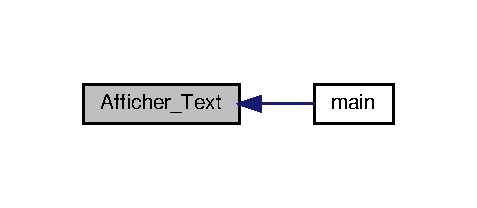
\includegraphics[width=229pt]{text_8h_a307b7655043a42402d751a3da90ff1d0_icgraph}
\end{center}
\end{figure}
\mbox{\Hypertarget{text_8h_aed94d72c6d43ac78f60f25e0d622d3bd}\label{text_8h_aed94d72c6d43ac78f60f25e0d622d3bd}} 
\index{text.\+h@{text.\+h}!free\+Font@{free\+Font}}
\index{free\+Font@{free\+Font}!text.\+h@{text.\+h}}
\subsubsection{\texorpdfstring{free\+Font()}{freeFont()}}
{\footnotesize\ttfamily void free\+Font (\begin{DoxyParamCaption}\item[{T\+T\+F\+\_\+\+Font $\ast$$\ast$}]{police }\end{DoxyParamCaption})}



Liberer la surface. 


\begin{DoxyParams}{Paramètres}
{\em police} & le font \\
\hline
\end{DoxyParams}
\begin{DoxyReturn}{Renvoie}
rien 
\end{DoxyReturn}
Voici le graphe des appelants de cette fonction \+:
\nopagebreak
\begin{figure}[H]
\begin{center}
\leavevmode
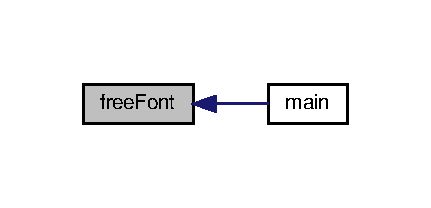
\includegraphics[width=207pt]{text_8h_aed94d72c6d43ac78f60f25e0d622d3bd_icgraph}
\end{center}
\end{figure}
\mbox{\Hypertarget{text_8h_a2dc500fe2665ba740d37f08e490c2a6a}\label{text_8h_a2dc500fe2665ba740d37f08e490c2a6a}} 
\index{text.\+h@{text.\+h}!init\+Temps@{init\+Temps}}
\index{init\+Temps@{init\+Temps}!text.\+h@{text.\+h}}
\subsubsection{\texorpdfstring{init\+Temps()}{initTemps()}}
{\footnotesize\ttfamily void init\+Temps (\begin{DoxyParamCaption}\item[{\hyperlink{structTime}{Time} $\ast$}]{time }\end{DoxyParamCaption})}



initialiser \hyperlink{structTime}{Time} time. 


\begin{DoxyParams}{Paramètres}
{\em time} & le \hyperlink{structTime}{Time} \\
\hline
\end{DoxyParams}
\begin{DoxyReturn}{Renvoie}
Rien 
\end{DoxyReturn}
Voici le graphe des appelants de cette fonction \+:
\nopagebreak
\begin{figure}[H]
\begin{center}
\leavevmode
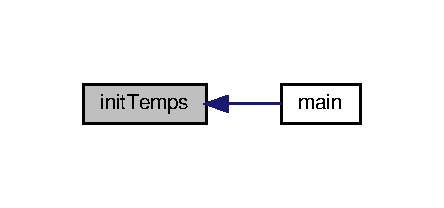
\includegraphics[width=213pt]{text_8h_a2dc500fe2665ba740d37f08e490c2a6a_icgraph}
\end{center}
\end{figure}
\mbox{\Hypertarget{text_8h_ab262a155d2f6fdeefc6ad6d63da93c82}\label{text_8h_ab262a155d2f6fdeefc6ad6d63da93c82}} 
\index{text.\+h@{text.\+h}!init\+Text@{init\+Text}}
\index{init\+Text@{init\+Text}!text.\+h@{text.\+h}}
\subsubsection{\texorpdfstring{init\+Text()}{initText()}}
{\footnotesize\ttfamily void init\+Text (\begin{DoxyParamCaption}\item[{\hyperlink{structText}{Text} $\ast$}]{T }\end{DoxyParamCaption})}



initialiser \hyperlink{structText}{Text} T. 


\begin{DoxyParams}{Paramètres}
{\em T} & le \hyperlink{structText}{Text} \\
\hline
\end{DoxyParams}
\begin{DoxyReturn}{Renvoie}
Rien 
\end{DoxyReturn}
Voici le graphe des appelants de cette fonction \+:
\nopagebreak
\begin{figure}[H]
\begin{center}
\leavevmode
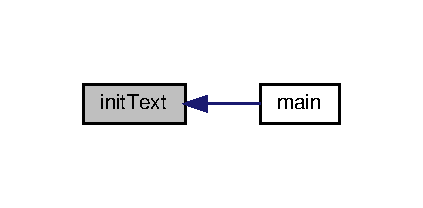
\includegraphics[width=203pt]{text_8h_ab262a155d2f6fdeefc6ad6d63da93c82_icgraph}
\end{center}
\end{figure}
\mbox{\Hypertarget{text_8h_a6f50df17af941d4d1aff8d62c336edca}\label{text_8h_a6f50df17af941d4d1aff8d62c336edca}} 
\index{text.\+h@{text.\+h}!load\+Font@{load\+Font}}
\index{load\+Font@{load\+Font}!text.\+h@{text.\+h}}
\subsubsection{\texorpdfstring{load\+Font()}{loadFont()}}
{\footnotesize\ttfamily void load\+Font (\begin{DoxyParamCaption}\item[{T\+T\+F\+\_\+\+Font $\ast$$\ast$}]{police }\end{DoxyParamCaption})}



Load Font. 


\begin{DoxyParams}{Paramètres}
{\em police} & le font \\
\hline
\end{DoxyParams}
\begin{DoxyReturn}{Renvoie}
Rien 
\end{DoxyReturn}
Voici le graphe des appelants de cette fonction \+:
\nopagebreak
\begin{figure}[H]
\begin{center}
\leavevmode
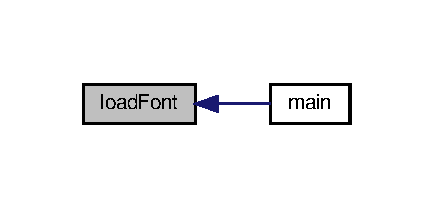
\includegraphics[width=208pt]{text_8h_a6f50df17af941d4d1aff8d62c336edca_icgraph}
\end{center}
\end{figure}

\hypertarget{voiture_8c}{}\section{Référence du fichier voiture.\+c}
\label{voiture_8c}\index{voiture.\+c@{voiture.\+c}}
{\ttfamily \#include $<$S\+D\+L/\+S\+D\+L.\+h$>$}\newline
{\ttfamily \#include $<$stdio.\+h$>$}\newline
{\ttfamily \#include \char`\"{}voiture.\+h\char`\"{}}\newline
{\ttfamily \#include \char`\"{}background.\+h\char`\"{}}\newline
{\ttfamily \#include \char`\"{}text.\+h\char`\"{}}\newline
Graphe des dépendances par inclusion de voiture.\+c\+:
\nopagebreak
\begin{figure}[H]
\begin{center}
\leavevmode
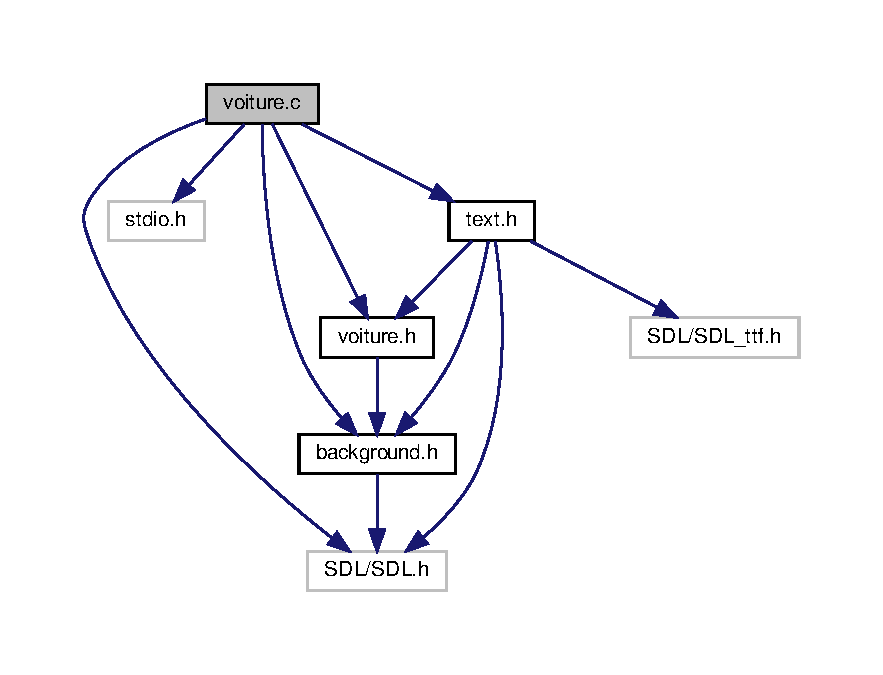
\includegraphics[width=350pt]{voiture_8c__incl}
\end{center}
\end{figure}
\subsection*{Fonctions}
\begin{DoxyCompactItemize}
\item 
void \hyperlink{voiture_8c_a20fdd4e4c29a45446e170697fdcd8df3}{load\+Voiture\+Images} (\hyperlink{structVoiture}{Voiture} $\ast$A)
\begin{DoxyCompactList}\small\item\em Load \hyperlink{structVoiture}{Voiture} A. \end{DoxyCompactList}\item 
void \hyperlink{voiture_8c_ac14144b9123d356bd28406e6d244ba09}{init\+Voiture} (\hyperlink{structVoiture}{Voiture} $\ast$A)
\begin{DoxyCompactList}\small\item\em initialiser \hyperlink{structVoiture}{Voiture} A. \end{DoxyCompactList}\item 
void \hyperlink{voiture_8c_a56efa82c5b16b51ee9da3cbc1075cde2}{move\+Voiture} (\hyperlink{structVoiture}{Voiture} $\ast$A, \hyperlink{structBackground}{Background} $\ast$B, Uint32 dt)
\begin{DoxyCompactList}\small\item\em Mouvement \hyperlink{structVoiture}{Voiture} A. \end{DoxyCompactList}\item 
void \hyperlink{voiture_8c_a4d5d4a48e7800b5768acf4b5b5ba6cf9}{free\+Voiture} (\hyperlink{structVoiture}{Voiture} $\ast$A)
\begin{DoxyCompactList}\small\item\em Liberer la surface. \end{DoxyCompactList}\end{DoxyCompactItemize}


\subsection{Documentation des fonctions}
\mbox{\Hypertarget{voiture_8c_a4d5d4a48e7800b5768acf4b5b5ba6cf9}\label{voiture_8c_a4d5d4a48e7800b5768acf4b5b5ba6cf9}} 
\index{voiture.\+c@{voiture.\+c}!free\+Voiture@{free\+Voiture}}
\index{free\+Voiture@{free\+Voiture}!voiture.\+c@{voiture.\+c}}
\subsubsection{\texorpdfstring{free\+Voiture()}{freeVoiture()}}
{\footnotesize\ttfamily void free\+Voiture (\begin{DoxyParamCaption}\item[{\hyperlink{structVoiture}{Voiture} $\ast$}]{A }\end{DoxyParamCaption})}



Liberer la surface. 


\begin{DoxyParams}{Paramètres}
{\em A} & la voiture \\
\hline
\end{DoxyParams}
\begin{DoxyReturn}{Renvoie}
rien 
\end{DoxyReturn}
Voici le graphe des appelants de cette fonction \+:
\nopagebreak
\begin{figure}[H]
\begin{center}
\leavevmode
\includegraphics[width=218pt]{voiture_8c_a4d5d4a48e7800b5768acf4b5b5ba6cf9_icgraph}
\end{center}
\end{figure}
\mbox{\Hypertarget{voiture_8c_ac14144b9123d356bd28406e6d244ba09}\label{voiture_8c_ac14144b9123d356bd28406e6d244ba09}} 
\index{voiture.\+c@{voiture.\+c}!init\+Voiture@{init\+Voiture}}
\index{init\+Voiture@{init\+Voiture}!voiture.\+c@{voiture.\+c}}
\subsubsection{\texorpdfstring{init\+Voiture()}{initVoiture()}}
{\footnotesize\ttfamily void init\+Voiture (\begin{DoxyParamCaption}\item[{\hyperlink{structVoiture}{Voiture} $\ast$}]{A }\end{DoxyParamCaption})}



initialiser \hyperlink{structVoiture}{Voiture} A. 


\begin{DoxyParams}{Paramètres}
{\em A} & la voiture \\
\hline
\end{DoxyParams}
\begin{DoxyReturn}{Renvoie}
Rien 
\end{DoxyReturn}
Voici le graphe des appelants de cette fonction \+:
\nopagebreak
\begin{figure}[H]
\begin{center}
\leavevmode
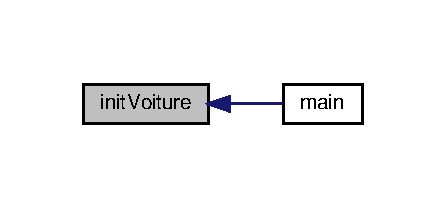
\includegraphics[width=214pt]{voiture_8c_ac14144b9123d356bd28406e6d244ba09_icgraph}
\end{center}
\end{figure}
\mbox{\Hypertarget{voiture_8c_a20fdd4e4c29a45446e170697fdcd8df3}\label{voiture_8c_a20fdd4e4c29a45446e170697fdcd8df3}} 
\index{voiture.\+c@{voiture.\+c}!load\+Voiture\+Images@{load\+Voiture\+Images}}
\index{load\+Voiture\+Images@{load\+Voiture\+Images}!voiture.\+c@{voiture.\+c}}
\subsubsection{\texorpdfstring{load\+Voiture\+Images()}{loadVoitureImages()}}
{\footnotesize\ttfamily void load\+Voiture\+Images (\begin{DoxyParamCaption}\item[{\hyperlink{structVoiture}{Voiture} $\ast$}]{A }\end{DoxyParamCaption})}



Load \hyperlink{structVoiture}{Voiture} A. 


\begin{DoxyParams}{Paramètres}
{\em A} & la voiture \\
\hline
\end{DoxyParams}
\begin{DoxyReturn}{Renvoie}
Rien 
\end{DoxyReturn}
Voici le graphe des appelants de cette fonction \+:
\nopagebreak
\begin{figure}[H]
\begin{center}
\leavevmode
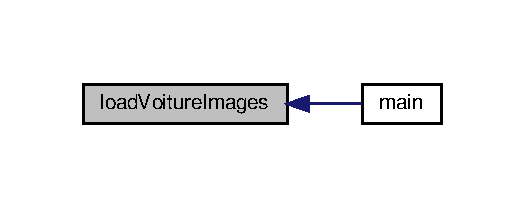
\includegraphics[width=252pt]{voiture_8c_a20fdd4e4c29a45446e170697fdcd8df3_icgraph}
\end{center}
\end{figure}
\mbox{\Hypertarget{voiture_8c_a56efa82c5b16b51ee9da3cbc1075cde2}\label{voiture_8c_a56efa82c5b16b51ee9da3cbc1075cde2}} 
\index{voiture.\+c@{voiture.\+c}!move\+Voiture@{move\+Voiture}}
\index{move\+Voiture@{move\+Voiture}!voiture.\+c@{voiture.\+c}}
\subsubsection{\texorpdfstring{move\+Voiture()}{moveVoiture()}}
{\footnotesize\ttfamily void move\+Voiture (\begin{DoxyParamCaption}\item[{\hyperlink{structVoiture}{Voiture} $\ast$}]{A,  }\item[{\hyperlink{structBackground}{Background} $\ast$}]{B,  }\item[{Uint32}]{dt }\end{DoxyParamCaption})}



Mouvement \hyperlink{structVoiture}{Voiture} A. 


\begin{DoxyParams}{Paramètres}
{\em A} & la voiture \\
\hline
{\em B} & the background \\
\hline
{\em dt} & variation dt \\
\hline
\end{DoxyParams}
\begin{DoxyReturn}{Renvoie}
Rien 
\end{DoxyReturn}
Voici le graphe des appelants de cette fonction \+:
\nopagebreak
\begin{figure}[H]
\begin{center}
\leavevmode
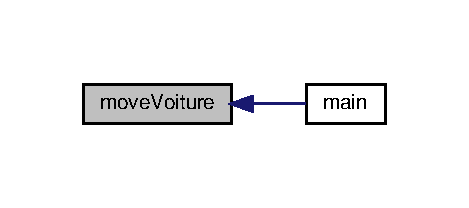
\includegraphics[width=225pt]{voiture_8c_a56efa82c5b16b51ee9da3cbc1075cde2_icgraph}
\end{center}
\end{figure}

\input{voiture_8h}
%--- End generated contents ---

% Index
\backmatter
\newpage
\phantomsection
\clearemptydoublepage
\addcontentsline{toc}{chapter}{Index}
\printindex

\end{document}
